\chapter{Fallstudie}

Es sollen zwei Ampeln nachgebaut werden, die  in einer experimentellen Umgebung die Funktionsweise realer Ampeln zeigen. Eine der Ampeln soll die gelbe LED blinken und die andere soll im normalen Betrieb sein. In diesem Projekt soll der CI/CD Methode von Development bis zum Deployment angewendet werden.

\section{Anforderungen}\label{anforderungen}

In diesem Abschnitt werden die funktionale und nicht-funktionale Anforderungen für die Realisierung des Projekts analysiert.


\subsection{Funktionale Anforderungen}

Die funktionalen Anforderungen beschreiben die gewünschte Funktionalität und das Verhalten des Systems, die in Tabelle\ref{funktionale} aufgelistet sind.


\begin{table}[h!]
	\begin{flushleft}
		{\small 
			\begin{tabular}{|c|c|}
				\hline
				Must-have & 
				\begin{minipage}{5in}
					 \begin{enumerate}
					 	\item Simulierung zwei Verkehrsampeln mithilfe von Raspberry Pi’s und LEDs
					 	\item Automatische Steuerung der LEDs durch GPIO Schnittstelle
					 	\item Entwicklung einer Software für das Blinken der gelben LED
					 	\item Entwicklung einer Software für den Normalbetrieb der Ampel
					 	\item Automatische Software-Test
					 	\item Automatische Bereitstellung (release) der Software
					 	\item Implementierung von \ac{CI/CD} Software-Entwicklungsmethode
					 \end{enumerate}
				\end{minipage} \\
				\hline
				Should-have & 
				\begin{minipage}{5in}
					\begin{enumerate}
						\item Automatische Containerisierung der für das Ampelsystem entwickelten Software mithilfe von Docker
						\item Automatische Veröffentlichung von containerisierten Software auf Docker Hub
						\item Orchestrierung der Docker-Containers mithilfe von Kubernetes
					\end{enumerate}
				\end{minipage} \\
				\hline
				Could-have & 
				\begin{minipage}{5in}
					\begin{enumerate}
						\item Automatische Übertragung (deploy) der Software an das Endgerät
					\end{enumerate}
				\end{minipage} \\
			\hline
			\end{tabular}	
		}
	\end{flushleft}
	\caption{Funktionale Anforderungen}\label{funktionale}
\end{table}



\subsection{Nicht-Funktionale Anforderungen}

Nicht-funktionale Anforderungen beschreiben die Qualität der oben genannten Funktionen, die erreicht werden müssen. Daher haben sie einen erheblichen Einfluss auf Ressourcenverbrauch, Entwicklung und Wartung. Darüber hinaus tragen diese Anforderungen dazu bei, die Akzeptanz des Systems zu verbessern. Einige dieser Anforderungen werden im Folgenden aufgelistet und erörtert.

\begin{itemize}
	\item \textbf{Zuverlässig:} Zuverlässigkeit stellt die Grundvoraussetzung für die Akzeptanz des Systems dar. Das korrekte Verhalten und der Übergang in einen sicheren Zustand im Fehlerfall muss immer gewährleistet sein. Falls die Übertragung der Software in einem inkorrekten Zustand endet, müssen Entwickler in der Lage sein, das System in den korrekten Zustand wiederherzustellen.
	\item \textbf{Skalierbar:} Das Projekt soll skalierbar sein. Wenn man eine neue Ampel nachbauen möchte, sollte es einfach und nicht kompliziert sein.
	\item \textbf{Fehlertoleranz:} Im Falle eines Fehlers sollte die Pipeline die weitere Ausführung anderer Schritte stoppen, wodurch Fehler vermieden werden, die aufgrund einer nachfolgenden Ausführung auftreten können.
	\item \textbf{Robust:} Der Pull-Request soll nicht gemergt werden, bevor die Fehlerfreiheit des Programms durch bestehenden Unit-Test bestätigt wird.
	\item \textbf{Zeiteffizient:} Der gesamte Prozess, von der Entwicklung bis zur Auslieferung, muss in kurzer Zeit und ohne Unterbrechung erfolgen.
	\item \textbf{Echtzeitüberwachung:} Während der Übertragung des Software-Updates soll dieses in Echtzeit überwacht werden.
	
\end{itemize}





\section{Konzept}


\subsection{Geeignete Software-Update-Strategie der Ampelanlage}

Heutzutage sind mehr Geräte mit dem Internet verbunden als je zuvor, was bedeutet, dass Software-Updates über das Internet und nicht über eine traditionelle Schnittstelle bereitgestellt werden müssen. Das spart viel Zeit und Geld bei der Wartung der Software und entlastet vor allem den Facharbeitern. Darüber hinaus wird die Fehlersuche im Fehlerfall durch den einfachen Fernzugriff auf das betroffene System erheblich vereinfacht. 
Diese Strategie wird als Softwar Over The Air (SOTA) benannt. Durch diese Strategie wird die Echtzeitüberwachung der Übertragung ermöglicht, was das ganze Software-Update der Ampelanlage übersichtlicher macht. Darüber hinaus wird durch SOTA Flexibilität bei der Software-Update erreicht, was bedeutet, dass jede Softwareversion mit einem einzigen Klick auf das System übertragen werden kann.
Dies macht die Strategie einfach zu handhaben. Neben all diesen Vorteilen hat das System noch einen weiteren Vorteil, nämlich die Anzahl der Updates ist nicht begrenzt und somit nicht zeitabhängig.


\subsection{Software Update-Architektur der Ampelanlage}

Um die oben genannten Vorteile nutzen zu können, ist es notwendig, eine Internet-Schnittstelle zur Außenwelt zu schaffen. In diesem Zusammenhang und aufgrund der im Raspberry Pi integrierten Internetschnittstelle eignet sich der Raspberry Pi für dieses System,  und weil es sich um ein Minicomputer handelt, erfüllt die in diesem Projekt aufgelistete Anforderungen. Die Abbildung \ref{fig:FW-Update-Strategie} zeigt, wie ein Entwickler, über das im Raspberry Pi integrierte Internetschnittstelle ein Update auf der Ampelanlage übertragen kann, nachdem er die Software auf GitLab hochgeladen hat. Die Verteilung der korrekten Software-Version an den entsprechenden Ampelanlage erfolgt über Raspberry Pis, die direkt mit den Ampelanlagen angeschlossen sind.
\newline\newline
Die Software-Update-Architektur in Abbildung\ref{fig:FW-Update-Strategie} zeigt deutlich, dass für die Anforderungen, die im Abschnitt \ref{anforderungen} aufgelistet sind, eine hierarchische Software-Deployment Topologie dafür geeignet ist. 
\newline\newline
Die Architektur von Kubernetes, die im Kapital {\LARGE ??} beschrieben wurde, bietet die Möglichkeit ein hierarchische Firmware-Deployment aufzubauen.


\begin{figure}[bth] 
	\centering
	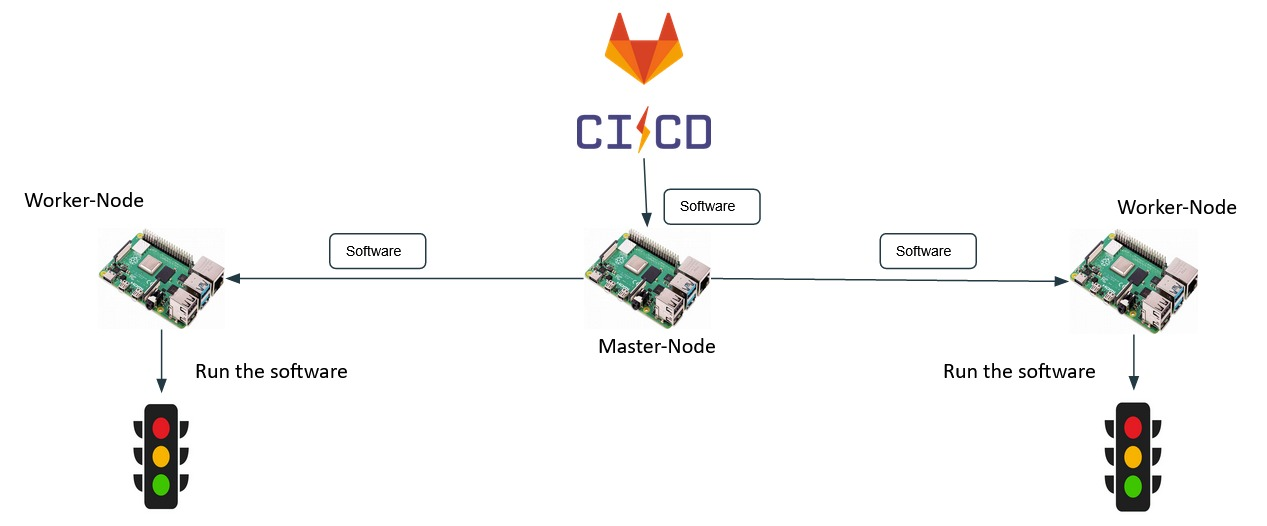
\includegraphics[width=0.7\textwidth]{Graphics/architektur.jpeg}
	\caption{Übersicht der Software Update}
	\label{fig:FW-Update-Strategie}
\end{figure}

\subsection{Auswahl der geeigneten Release-Managementmethode}

Die Unterschiede der Release-Managementmethoden zeigen, dass die CD-Methode es ermöglicht, qualitativ hochwertige Software-Release in kurze Zeit auf einem Endgerät zu übertragen. CD Methode bietet automatisierte Build- , Test- und Deploymentschritte, um vom Menschen verursachte Fehler zu vermeiden, die bei der manuellen Durchführung der Phasen auftreten können. Außerdem können in jeder Phase Probleme auftreten. Abhängigkeiten zwischen den Schritten können eine schnelle Fehlerkorrektur garantieren. Tritt in einer Phase ein Fehler auf, wird die Pipeline unterbrochen und somit weitere Fehler verhindert. Die Software kann nahtlos, sicher, zuverlässig und wiederholt auf dem Endgerät übertragen werden. Darüber hinaus kann der Entwickler den Fortschritt der Phasen beobachten, was hilft, wenn während der Phase ein Fehler auftritt, kann der Entwickler nur ab dieser Phase und nicht von allen Phasen aus iterieren. Bei anderen Release-Managementmethoden benötigen Produkthersteller Releasemanager, um Entscheidungen darüber zu treffen, wann Releases erstellt werden, wie einzelne Schritte ausgeführt werden und wann Software ausgeliefert werden soll. Die Methode CD ermöglicht es dem Release Manager, sich mehr auf die operative Seite zu konzentrieren, wie beispielsweise die Erstellung eines automatisierten Prozesses und Workflows zur sicheren Migration von Code in das Endprodukt, anstatt sich auf die Planungs-, Entwicklungs- und Testphasen zu konzentrieren.



\subsection{Auswahl der geeigneten Release-Strategie}

Die Wahl einer geeigneten Release-Strategie hängt vom Hersteller des Produkts und dem Produkt selbst ab. Bei modernen medizinischen Geräten, Fahrzeuge und IoT Geräte sind Fehlerbehebung und neue Funktionen für einen besseren Service für die Kunden unerlässlich. Daher wird in dieser Fallstudie eine flexible Release-Strategie bevorzugt. Die Schritte im Release-Management-Prozess bleiben generisch, sodass der Wechsel zu anderen Release-Strategien einfach sein kann. Eine flexible Release-Strategie sieht laut Dr.-Ing. Kühn in der Regel die Planung von Änderungen an einem bestimmten Produkt vor\cite{doktor-thesis}.





\section{Entwicklungsvorgang}



\section{Implementierung}

